\chapter{Implementation}
In this chapter we describe implementation of Giflang and provide insights into the decisions we made along the way. As Figure \ref{fig:chap4:overview} shows,
the project consists of two major parts: an interpreter and a web IDE. These two components can be found in the \texttt{interpreter/} and the \texttt{frontend/}
folders, respectively. The Figure \ref{fig:chap4:overview} also outlines the API of the interpreter that allows the web IDE to execute user's programs.
This API is further discussed in subsection /TODO/
\begin{figure}[!hbt]
    \centering
    \label{fig:chap4:overview}
    \tikzset{every picture/.style={line width=0.75pt}} %set default line width to 0.75pt        
    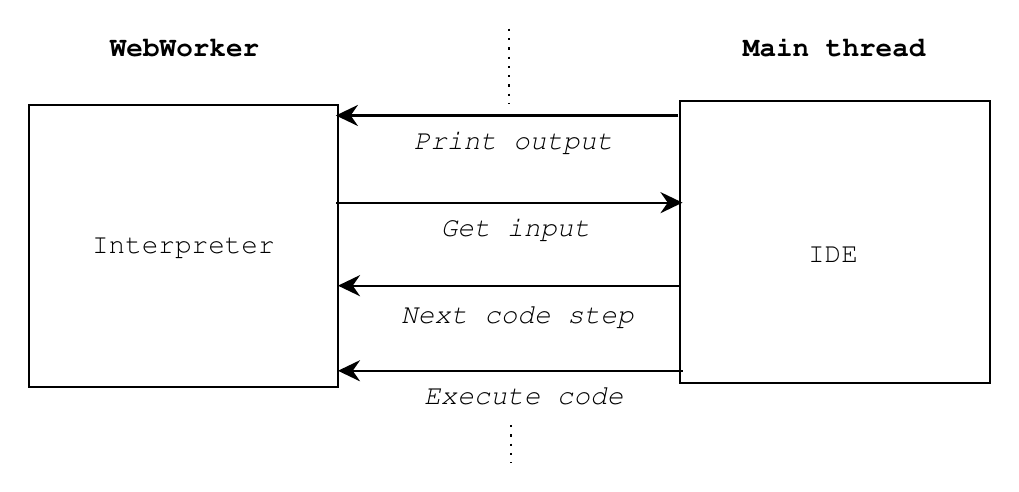
\begin{tikzpicture}[x=0.75pt,y=0.75pt,yscale=-1,xscale=1]
    \draw   (37.5,92) -- (186.5,92) -- (186.5,228) -- (37.5,228) -- cycle ;
    \draw    (352.5,220) -- (189.5,220) ;
    \draw [shift={(186.5,220)}, rotate = 360] [fill={rgb, 255:red, 0; green, 0; blue, 0 }  ][line width=0.08]  [draw opacity=0] (10.72,-5.15) -- (0,0) -- (10.72,5.15) -- (7.12,0) -- cycle    ;
    \draw    (351.5,179) -- (189.5,179) ;
    \draw [shift={(186.5,179)}, rotate = 360] [fill={rgb, 255:red, 0; green, 0; blue, 0 }  ][line width=0.08]  [draw opacity=0] (10.72,-5.15) -- (0,0) -- (10.72,5.15) -- (7.12,0) -- cycle    ;
    \draw    (349.5,139) -- (185.5,139) ;
    \draw [shift={(352.5,139)}, rotate = 180] [fill={rgb, 255:red, 0; green, 0; blue, 0 }  ][line width=0.08]  [draw opacity=0] (10.72,-5.15) -- (0,0) -- (10.72,5.15) -- (7.12,0) -- cycle    ;
    \draw    (350.5,97) -- (188.5,97) ;
    \draw [shift={(185.5,97)}, rotate = 360] [fill={rgb, 255:red, 0; green, 0; blue, 0 }  ][line width=0.08]  [draw opacity=0] (10.72,-5.15) -- (0,0) -- (10.72,5.15) -- (7.12,0) -- cycle    ;
    \draw  [dash pattern={on 0.84pt off 2.51pt}]  (269,55.2) -- (269,91.2) ;
    \draw  [dash pattern={on 0.84pt off 2.51pt}]  (270,246.2) -- (270,264.2) ;
    \draw   (351.5,90) -- (500.5,90) -- (500.5,226) -- (351.5,226) -- cycle ;
    \draw (425,164) node   [align=left] {{\fontfamily{pcr}\selectfont IDE}};
    \draw (112.02,161) node   [align=left] {{\fontfamily{pcr}\selectfont Interpreter}};
    \draw (112.6,64.4) node  [font=\normalsize] [align=left] {{\fontfamily{pcr}\selectfont \textbf{WebWorker}}};
    \draw (425.6,64.4) node  [font=\normalsize] [align=left] {{\fontfamily{pcr}\selectfont \textbf{Main thread}}};
    \draw (276.02,232) node   [align=left] {{\fontfamily{pcr}\selectfont \textit{Execute code}}};
    \draw (273.02,194) node   [align=left] {{\fontfamily{pcr}\selectfont \textit{Next code step}}};
    \draw (272.02,152) node   [align=left] {{\fontfamily{pcr}\selectfont \textit{Get input}}};
    \draw (271.02,110) node   [align=left] {{\fontfamily{pcr}\selectfont \textit{Print output}}};
    \end{tikzpicture}
    \caption{A high-level diagram of the implementation}
\end{figure}

\section{Interpreter}
Every interpreter first \emph{parses} a source code and then \emph{executes} the parsed tree (Fig \ref{fig:chap4:interpreter}). There is a room for a lot of optimizations along the way in order
to make the execution as fast as possible. However, we do not incorporate any optimizations into the interpreter and only execute the parsed tree node by node.

\begin{figure}[!hbt]
    \centering
    \label{fig:chap4:interpreter}
    \tikzset{every picture/.style={line width=0.75pt}} %set default line width to 0.75pt        

    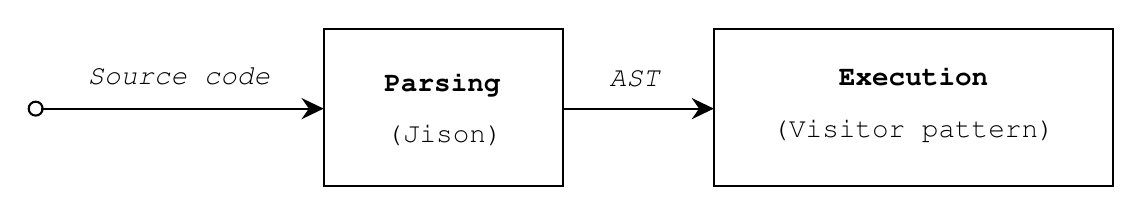
\begin{tikzpicture}[x=0.75pt,y=0.75pt,yscale=-1,xscale=1]
    %uncomment if require: \path (0,622); %set diagram left start at 0, and has height of 622

    %Shape: Rectangle [id:dp28122229657926034] 
    \draw   (226.5,34) -- (341.5,34) -- (341.5,110) -- (226.5,110) -- cycle ;
    %Straight Lines [id:da9888936135364137] 
    \draw    (411.25,72.5) -- (341.5,72.5) ;

    \draw [shift={(414.25,72.5)}, rotate = 180] [fill={rgb, 255:red, 0; green, 0; blue, 0 }  ][line width=0.08]  [draw opacity=0] (10.72,-5.15) -- (0,0) -- (10.72,5.15) -- (7.12,0) -- cycle    ;
    %Shape: Rectangle [id:dp7793277711435098] 
    \draw   (414.5,34) -- (606.5,34) -- (606.5,110) -- (414.5,110) -- cycle ;
    %Straight Lines [id:da7940866772557511] 
    \draw    (223.25,72.5) -- (89.85,72.5) ;
    \draw [shift={(87.5,72.5)}, rotate = 180] [color={rgb, 255:red, 0; green, 0; blue, 0 }  ][line width=0.75]      (0, 0) circle [x radius= 3.35, y radius= 3.35]   ;
    \draw [shift={(226.25,72.5)}, rotate = 180] [fill={rgb, 255:red, 0; green, 0; blue, 0 }  ][line width=0.08]  [draw opacity=0] (10.72,-5.15) -- (0,0) -- (10.72,5.15) -- (7.12,0) -- cycle    ;

    % Text Node
    \draw (283.5,61) node   [align=left] {{\fontfamily{pcr}\selectfont \textbf{Parsing}}};
    % Text Node
    \draw (510.5,57) node   [align=left] {{\fontfamily{pcr}\selectfont \textbf{Execution}}};
    % Text Node
    \draw (376.5,58) node   [align=left] {{\fontfamily{pcr}\selectfont \textit{AST}}};
    % Text Node
    \draw (284.5,85) node   [align=left] {{\fontfamily{pcr}\selectfont (Jison)}};
    % Text Node
    \draw (510.5,83) node   [align=left] {{\fontfamily{pcr}\selectfont (Visitor pattern)}};
    % Text Node
    \draw (156.5,57) node   [align=left] {{\fontfamily{pcr}\selectfont \textit{Source code}}};
    \end{tikzpicture}
    \caption{A diagram of the Giflang interpreter}
\end{figure}

\subsection{Parsing}
Parser is an interpreter component that checks whether the input source conforms to the rules of the formal grammar of a language. Additionally, parsers help
building an AST from the source code. In the very beginning of this thesis we briefly explained what grammar rules and AST is (see Fig \ref{fig:chap1:tokens_and_grammar})

Parsers usually consist of two separate parts: \emph{lexing} or \emph{tokenization} and \emph{parsing}. A lexer splits input text into \emph{tokens}.
For example it can split an input \texttt{'4 + size'} into following tokens:
\begin{code}
// Sample tokens for an input '4 + size'
[{ "Type": "NUMBER", "Text": "4" },
 { "Type": "OPERATOR", "Text": "+" },
 { "Type": "IDENTIFIER", "Text": "size" }]
\end{code}

Grammar rules are then defined in terms of tokens, for example:
\begin{figure}[!hbt]
\begin{code}
expression -> factor OPERATOR expression
expression -> factor
factor -> IDENTIFIER
factor -> NUMBER
\end{code}
    \caption{An example of a grammar definition}
    \label{fig:chap4:grammar}
\end{figure}

The grammar above defines a language consisting of expressions that can contain numbers and identifiers. It is very minimal as it does not account
for operator precedence or parenthesis. Lowercase words are \emph{nonterminals} and capitalized words are \emph{terminals}. Terminal symbols are elementary
symbols and can not be replaced by other terminals or nonterminals. Nonterminals can appear on the left side of productions and they are replaced by groups
of terminal symbols according to the production rules.

In order to parse a grammar like the one above, we can either create our own parser or use \emph{a parser generator}. We will briefly describe both options.
There are many ways of creating a custom parser, but we will discuss the most common one, a recursive-descent parser. Parsers are a large topic and
we do not intent to dive deep into it.

\subsubsection*{Recursive-descent parser}
A recursive-descent parser is a method of creating a parser using mutually recursive procedures where each procedure implements one of the nonterminals
of the grammar. To give us a better idea of what it means to create a function for each nonterminal, we created a parser for the grammar from
the Figure \ref{fig:chap4:grammar} in Python.
\begin{code}
# Unimplemented functions:
#   * curToken -- returns the current token
#   * nextToken -- advances to the next token

def accept(token):
    if curToken() == token:
        nextToken()
        return 1
    return 0

def expect(token):
    if accept(token):
        return 1
    raise Exception("expect: unexpected token")

def factor():
    if accept('IDENTIFIER'):
        # Action
        pass
    elif accept('NUMBER'):
        # Action
        pass 
    else:
        raise Exception("factor: syntax error")

def expression():
    factor()
    if accept('OPERATOR'):
        expression()
        # Action
        return
    # Action 
\end{code}

We can see that the grammar can be transformed into the code very naturally using a recursive-descent parser. The \texttt{'\# Action'} comments mark places where
grammar rules are applied and we could add bits of code there that would build a derivation tree.

Recursive-descent parsers can run in linear time with respect to the input string size, granted that the parsed grammar is an LL(k). \emph{An LL(k) grammar} is
a context-free grammar that is parsed by an LL parser, which parses the input from \textbf{L}eft to right and creates a \textbf{L}eftmost derivation.
Additionally, it requires at most $k$ lookahead tokens to uniquely identify which rule should be applied next.

\subsubsection*{Parser generators}
Creating parsers can be a repetitive process -- applying the same patterns to different grammars. Parser generators solve this by generating parsers from grammar
specifications. There are dozens of parser generators, but we will only describe one of them, GNU Bison/TODO cite/.

We will also use Flex in the examples, a lexical analyzer generator that is often used alongside Bison. Both Flex and Bison can target C, C++, and Java.

Flex takes token descriptions as regular expressions. The following code is not a valid Flex source, but it demonstrates the idea behind Flex:
\begin{code}
%{ %}

DIGIT           [0-9]
LETTER          [a-zA-Z]

%%
{DIGIT}+                        return NUMBER;
{LETTER}({LETTER}|{DIGIT})*     return IDENTIFIER;
[+-]                            return OPERATOR;
%%
\end{code}

Flex can create a lexer from the source code above. Let us now show a Bison source for the grammar from the Figure \ref{fig:chap4:grammar}:
\begin{code}
%{ %}

%token NUMBER IDENTIFIER OPERATOR
%start expression

%%
expression
    : factor OPERATOR expression    { /* Action */ }
    | factor                        { /* Action */ }
    ;
factor
    : IDENTIFIER                    { /* Action */ }
    | NUMBER                        { /* Action */ }
    ;
%%
\end{code}

Parse generators can employ many different parsing algorithms, but the most common ones are LL parser and LALR, as it is also case with Bison. We will not describe
the mentioned parsers since we do not find it important in our case.

\subsubsection*{Conclusion}
The main advantage of creating a custom parser over a parser generator is the option to create better error reporting and error recovery. It would also be a
good learning experience to make a parser with a lexer from scratch. However, we opted for using a parser generator as in the very beginning of the project
we wanted to focus on interpreting the AST rather than parsing.

There are numerous parser generators for JavaScript, most notably ANTLR and acorn /TODO cite/. Since we had prior experience with Bison, we decided to use
Jison /TODO cite/, a Bison-like JavaScript library. The Jison source file location is \texttt{interpreter/ast/giflang.jison}.

\subsection{Employing the Visitor pattern}
Probably the easiest way to create an interpreter is by using \emph{the interpreter design pattern}. The basic idea is to have a class for each symbol
(terminal or nonterminal). The syntax tree is then build from these classes. Every class defines an \texttt{evaluate} method that interprets given node
of the syntax tree, possibly evaluating its children nodes as well.

Below is a Python example of the interpreter pattern that evaluates the grammar from the Figure \ref{fig:chap4:grammar}. We did not define a class for each
symbol to make it more concise.
\begin{code}
class Node:
    def evaluate(self, env):
        raise Exception('Method not implemented')

class Expression(Node):
    def __init__(self, left, right, op):
        self.left, self.right, self.op = left, right, op

    def evaluate(self, env):
        lval, rval = self.left.evaluate(env), self.right.evaluate(env)
        if self.op == '+':
            return lval + rval
        elif self.op == '-':
            return lval - rval
        else:
            raise Error('Unknown operator ' + self.op)

class Number(Node):
    def __init__(self, value):
        self.value = value
    
    def evaluate(self, env):
        return self.value

class VariableAccess(Node):
    def __init__(self, identifier):
        self.identifier = identifier
    
    def evaluate(self, env):
        if self.identifier in env:
            return env[self.identifier]
        else:
            raise Error('Unknown variable ' + self.identifier)

# Expression: 2 + x - 9
exp = Expression(
    Number(2),
    Expression(VariableAccess('x'), Number(9), '-'),
    '+')
# Prints 3
print(exp.evaluate({'x': 10}))
\end{code}

When using the interpreter pattern, the execution logic in the form of \texttt{evalute} methods is spread among multiple classes. In order to couple the
logic together we decided to use the visitor pattern. The visitor pattern /TODO/
\begin{code}
class Node:
    def accept(self, visitor):
        raise Exception('Method not implemented')

class Expression(Node):
    def __init__(self, left, right, op):
        self.left, self.right, self.op = left, right, op

    def accept(self, visitor):
        return visitor.visitExpression(self)

# We omit implementation of Number and VariableAccess nodes as
# they are very similar to the Expression node, i.e., they only
# define an accept method.

class Interpreter:
    def __init__(self, env):
        self.env = env
    
    def visitExpression(self, exprNode):
        lval = exprNode.left.accept(self)
        rval = exprNode.right.accept(self)
        if exprNode.op == '+':
            return lval + rval
        elif exprNode.op == '-':
            return lval - rval
        else:
            raise Error('Unknown operator ' + exprNode.op)
    
    def visitNumber(self, numberNode):
        return numberNode.value
    
    def visitVariableAccess(self, variableAccessNode):
        id = variableAccessNode.identifier
        if id in self.env:
            return self.env[id]
        else:
            raise Error('Unknown variable ' + id)

# Expression: 2 + x - 9
exp = Expression(
    Number(2),
    Expression(VariableAccess('x'), Number(9), '-'),
    '+')
interpreter = Interpreter({'x': 10})
# Prints 3
print(exp.accept(interpreter))
\end{code}

In the example above, the Interpreter class is a Visitor and its methods implement the execution logic.

The types of return values of different nodes might be different. When implementing the interpreter we found three different return types:
\begin{enumerate}
    \item \emph{An instance} -- for example literal or expression nodes return an instance
    \item \emph{An instance reference} -- accesing a variable, a property, or an array element has to result in an assignable value (i.e., a reference)
    \item \emph{A completion} -- cycles can contain \texttt{break} or \texttt{continue} statements that do not result in an instance, but rather a completion
\end{enumerate} 

In the implementation, we split the nodes into three categories based on their return types: \texttt{ValueExpr}, \texttt{RefExpr}, and \texttt{Stmt}.
The node classes can be found in \texttt{interpreter/ast/\{expr, stmt\}.ts}, and the interpreter visitor in \texttt{interpreter/interpreter.ts}. 

\subsection{Class hierarchy of the object model}
In the Section \ref{chap3:object_model} we outlined the object model of Giflang. In order to implement it in a statically-typed language like TypeScript, we
need to define a class hierarchy that will represent the object model. Since everything is an object, everything has to derive from a single class. We named
this class \texttt{Instance}.
\begin{figure}[!hbt]
	\includegraphics[width=1\textwidth]{../img/class_hierarchy}
	\label{fig:chap4:class_hierarchy}
    \caption{Class hierarchy of the object model}
\end{figure}

Classes \texttt{Instance} and \texttt{Class} are \emph{abstract}. As we can see from the Figure \ref{fig:chap4:class_hierarchy}, classes have their
respective instance classes; for example there is \texttt{NumberClass} and \texttt{NumberInstance}. This results in creating a relatively big number
of classes, but we did not find any other suitable model, because different classes of instances need to hold different value types. To illustrate this,
a \texttt{Number} need to hold a number, while \texttt{String} needs to hold a string, etc.

We could create a templated \texttt{Instance<T>} class that would have a \texttt{value: T} property. This way, we would be able to reduce the number of
classes. However, some of the instance classes also incorporate additional functionality, e.g., \texttt{UserFunctionInstance} implements a \texttt{call} method
that allows calling the function. Since there are more cases like this one, we decided to create all instances in a uniform fashion and did not go with the
generic \texttt{Instance<T>} approach.

Classes define their methods as static functions and during their initialization these methods are assigned to the class objects they represent.
A code snippet below demonstrates this:
\begin{code}
class NumberClass extends Class {
    // Overloads '+' operation of two numbers.
    static __add__(
        args: Instance[],
    ): NumberInstance {
        CheckArity(args, /* expectedArity = */ 2)
        const lhs = args[0].castOrThrow(NumberInstance)
        const rhs = args[1].castOrThrow(NumberInstance)
        return new NumberInstance(
            /* klass = */ NumberClass.get(), lhs + rhs)
    }

    constructor() {
        this.fields.set(
            /* fieldName = */ '__add__',
            new WrappedFunctionInstance(
                /* klass = */ WrappedFunctionClass.get(),
                NumberClass.__add__,
                /* functionName = */ '__add__'
            )
        )
    }
}
\end{code}

Since \texttt{NumberClass.\_\_add\_\_} is a TypeScript function it needs to be wrapped around Giflang's object. We named this wrapper a \texttt{WrappedFunctionInstance}.
The code in the actual implementation is a little more abstract since repeating this for every operation would need a lot of boilerplate.

When writing the code, we often needed the class objects, usually for instantiation. This can be seen in the code example above, e.g.,
\texttt{new NumberInstance(NumberClass.get(), lhs + rhs)}. In this case, \texttt{NumberClass.get()} is a \texttt{NumberClass} instance. Since only one
instance of each class object is needed, we used \emph{the singleton pattern}. In hindsight, it was not the best choice, because it allows changing
the interpreter state in between multiple invocations.
\begin{code}
const interpreter1 = new Interpreter()
// This code can change state of the singletons, for example
// override __add__ operation on the NumberClass.
interpreter1.visitProgramStmt(ParseGiflang('"evil" source code'))

const interpreter2 = new Interpreter()
// The second interpreter uses the same singletons and hence
// their state will be changed.
interpreter2.visitProgramStmt(ParseGiflang('source code'))
\end{code}

However, since we spawn a new WebWorker with each code run, this was not an issue. If we decide to reuse the same WebWorker, we can use a global registry
instead of singletons. Class objects in the registry can then be reinstantiated after each code execution.

\subsection{Environment state}

\subsection{Auxiliary letters}

\subsection{Code stepping (debugger)}

\subsection{Additive input}

\subsection{API}

\section{IDE}

\subsection{Choosing image format}

\subsection{State management (Redux)}

\subsection{Layout}